\documentclass[12pt]{article}

\usepackage[utf8]{inputenc}
\usepackage[T1]{fontenc}
\usepackage{lmodern}
\usepackage[margin=1in]{geometry}
\usepackage{setspace}
\usepackage{amsmath}
\usepackage{amssymb}
\usepackage{graphicx}
\usepackage{xcolor}
\usepackage{booktabs}
\usepackage{threeparttable}
\usepackage{caption}
\usepackage{microtype}
\usepackage[authoryear]{natbib}
\usepackage[colorlinks=true, linkcolor=blue!50!black, citecolor=blue!50!black, urlcolor=blue!50!black]{hyperref}

\providecommand{\sym}[1]{\ifmmode^{#1}\else\(^{#1}\)\fi}
\captionsetup{font=small, labelfont=bf}
\graphicspath{{../Figures/}}
\onehalfspacing

\title{Generative AI Exposure and House Prices:\\ Evidence from Danish Municipalities\thanks{All data are public, and the code that downloads and processes them accompanies the paper (Appendix~\ref{app:data}).}}
\author{}
\date{Draft, October 2026}

\begin{document}

\maketitle

\begin{abstract}
\noindent Generative artificial intelligence may change the expected earnings of workers whose tasks it can perform, and house prices should capitalize such changes where those workers live. I test this prediction for the 98 Danish municipalities, combining quarterly house prices with a measure of resident exposure built from the International Labour Organization's 2025 occupational exposure index and public Danish employment data. Across all municipalities, a one standard deviation increase in exposure is associated with 3.5 log points faster growth in house prices per square metre between 2022 and 2026, against average growth of 8.0 log points. The same gradient appears in 2015--2019, years before ChatGPT. Within provinces, the post-2022 association falls to 0.8 log points with a standard error of 1.0, and an event study shows no break in relative prices around the release of ChatGPT. The evidence is consistent with a long-running premium for educated urban municipalities rather than a response to generative AI, and it rules out within-province effects larger than about 3 log points per standard deviation.

\bigskip
\noindent \textbf{JEL:} J24, O33, R21, R31\\
\noindent \textbf{Keywords:} generative AI, occupational exposure, house prices, local labor markets
\end{abstract}

\newpage

%-------------------------------------------------------------------------------
\section{Introduction}
%-------------------------------------------------------------------------------

The public release of ChatGPT on 30 November 2022 made a general-purpose generative AI tool available to any worker with an internet connection. Task-based assessments suggest that such tools can perform a large share of the tasks in clerical, professional and technical occupations \citep{eloundou2024, gmyrek2023, gmyrek2025}. Controlled studies find large productivity gains in writing and customer support \citep{noy2023, brynjolfsson2025}. Yet the first evidence from administrative data finds small effects on earnings and hours so far \citep{humlum2025}. When realized earnings have not yet moved, forward-looking asset prices offer a way to see how markets assess who gains and who loses. \citet{eisfeldt2023} show that firms whose workforces were more exposed to generative AI earned higher stock returns after ChatGPT's release.

Housing is the largest asset for most households, and its price capitalizes the expected income of the people who want to live in a place \citep{roback1982, moretti2011, notowidigdo2020}. If generative AI raises the expected earnings of exposed workers, demand for housing should rise where those workers live, and prices should rise most where housing supply is inelastic \citep{glaeser2008, saiz2010}. If the technology instead substitutes for exposed workers, the same logic predicts slower price growth. This paper asks which pattern, if either, appears in the Danish housing market.

I build a measure of exposure to generative AI for each of the 98 Danish municipalities from public data. The measure starts from the International Labour Organization's 2025 exposure scores for ISCO-08 occupations \citep{gmyrek2025}. Danish occupation codes extend ISCO-08, so the scores apply without a crosswalk. Public Statistics Denmark tables do not report occupations by municipality. I therefore pass the scores through the occupation mix of each industry and skill level and weight the resulting cell scores by the 2017--2019 employment of each municipality's residents. I combine the measure with quarterly prices per square metre from Finans Danmark and compare price growth across municipalities before and after the release of ChatGPT.

Across all municipalities, house prices grew faster where exposure was higher. A one standard deviation increase in exposure is associated with 3.5 log points faster growth in the price per square metre of houses from the year before ChatGPT to the year ending in 2026Q2, a period in which prices grew by 8.0 log points on average. This association does not reflect a response to generative AI. The same regression for 2015--2019 yields 3.4 log points. Exposure correlates 0.94 with the 2019 price level and 0.92 with the share of residents with a tertiary degree, so it largely tracks the long-running premium of educated urban municipalities. When I compare municipalities within the same province, the post-ChatGPT association falls to 0.8 log points with a standard error of 1.0, and the 2015--2019 placebo association falls to 0.1 log points. An event study with province-by-quarter fixed effects shows no break in relative prices around the release of ChatGPT. Without province effects, the event-study coefficients follow a trend that starts well before 2022 and flattens afterward.

These results do not support the hypothesis that greater exposure to generative AI raised house price growth through mid-2026. They also do not rule out a smaller effect. Within provinces, the 95 percent confidence interval excludes effects above 2.7 log points per standard deviation of exposure, about a third of average price growth over the period. Two features of the design limit what the data can show. Provinces approximate regional labor markets, so the within-province comparison captures differences in where exposed workers live rather than shocks to regional labor demand. And the exposure measure misses differences in occupation mix within industry and skill cells, which biases estimates toward zero.

The paper contributes to three literatures. First, it extends the evidence on the economic effects of generative AI, which so far centres on productivity, labor markets and firm values \citep{noy2023, brynjolfsson2025, humlum2025, eisfeldt2023}, to the housing market. Second, it relates to work on how local labor demand shocks capitalize into house prices \citep{moretti2011, notowidigdo2020} and to regional exposure designs for trade, robots and earlier generations of AI \citep{autor2013, acemoglu2020robots, acemoglu2022ai}. Third, it documents a measurement problem for regional designs based on generative AI exposure. Exposed occupations concentrate in educated, high-price urban areas, which have experienced faster house price growth for other reasons. Exposure measures built from employment shares inherit the identifying assumptions of those shares \citep{goldsmithpinkham2020, borusyak2022}, and here the shares are nearly collinear with urban characteristics.

Section~\ref{sec:background} describes generative AI exposure, the channels through which it could affect house prices, and the Danish housing market after 2022. Section~\ref{sec:data} presents the data, and Section~\ref{sec:exposure} constructs the exposure measure. Section~\ref{sec:strategy} sets out the empirical strategy, Section~\ref{sec:results} reports the results, and Section~\ref{sec:discussion} discusses their interpretation and the next steps. Section~\ref{sec:conclusion} concludes.

%-------------------------------------------------------------------------------
\section{Background}\label{sec:background}
%-------------------------------------------------------------------------------

\subsection{Occupational exposure to generative AI}

The exposure scores in this paper come from the refined global index of \citet{gmyrek2025}. The index scores 3,265 tasks in 427 ISCO-08 unit groups on a scale from 0, for tasks that current generative AI cannot perform, to 1, for tasks it could perform entirely. Two large language models predict each task score, and experts reconcile disputed cases. The score of an occupation is the mean of its task scores. The index measures technical potential. It does not predict job loss, and an exposed occupation may gain or lose from the technology.

Exposure concentrates in clerical work. Data entry clerks, typists and accounting clerks have the highest occupation scores in the index, between 0.64 and 0.70. Professionals and technicians score in the middle of the distribution, and manual and elementary occupations score lowest. The 2023 version of the index \citep{gmyrek2023} also classifies occupations by whether generative AI is more likely to augment or to automate their tasks. I use this classification in Section~\ref{sec:discussion}. Other measures of AI exposure, based on abilities, patents or language-model ratings of tasks, produce broadly similar rankings of occupations \citep{felten2021, webb2020, eloundou2024}.

\subsection{Why house prices could respond}

In a spatial equilibrium, the price of housing in municipality $m$ equals the discounted value of the rents that residents are willing to pay,
\begin{equation}
P_{mt} = \mathbb{E}_t \sum_{s=0}^{\infty} \frac{R_{m,t+s}}{(1+r_t)^s},
\end{equation}
and rents rise with the income of the households who compete for housing there \citep{roback1982, moretti2011}. A technology that raises the expected earnings of some occupations shifts housing demand toward the places where those workers live and work. How much of the shift appears in prices depends on the elasticity of housing supply \citep{glaeser2008, saiz2010}. Because prices capitalize expectations, they can respond before earnings do.

The sign of the response is an empirical question. If generative AI complements exposed workers, their expected earnings rise and so does housing demand where they live. If it substitutes for them, expected earnings and housing demand fall. Two geographic channels are also worth separating. A shock to the earnings of exposed workers changes labor demand in regional labor markets as a whole, which affects all municipalities within commuting distance. The same shock also changes the relative demand for housing in the municipalities where exposed workers choose to live. Comparisons within provinces, which approximate regional labor markets, isolate the second channel.

\subsection{The Danish housing market after 2022}

Three macroeconomic events overlap with the arrival of generative AI and affect municipalities differently. First, Danmarks Nationalbank, which maintains the krone's peg to the euro, raised its policy rate from July 2022 in step with the European Central Bank, and long-term fixed mortgage rates rose by several percentage points during 2022. House prices fell in the second half of 2022. Municipalities with high prices relative to income are more sensitive to interest rates, and these are also the most exposed municipalities. Second, a new property valuation and taxation system took effect on 1 January 2024, which changed tax burdens differently across price levels. Third, the central bank began lowering its policy rate in June 2024. Any comparison of exposed and less exposed municipalities after 2022 must separate these forces from generative AI.

%-------------------------------------------------------------------------------
\section{Data}\label{sec:data}
%-------------------------------------------------------------------------------

All data are public. Table~\ref{tab:sources} in Appendix~\ref{app:data} lists the sources.

\paragraph{House prices.} The main outcome comes from table BM010 of Finans Danmark, which reports the average price per square metre of completed transactions by municipality and quarter. The table covers detached and terraced houses, owner-occupied flats and holiday homes from 1992Q1 to 2026Q2 and reports initial listing prices, final listing prices and realized transaction prices. I use realized prices for houses as the main outcome and flats as a secondary outcome. House prices are available for all 98 municipalities in almost every quarter since 2010, with 25 missing observations out of 4,508 between 2015Q1 and 2026Q2. Flat prices are missing for many rural municipalities, leaving 73 municipalities with a price change for flats between 2022 and 2026. The price per square metre is an average rather than a quality-adjusted index, so changes in the size or quality of the homes sold also move it.

\paragraph{Employment and occupations.} Statistics Denmark's register-based labor force statistics report employment at the end of November by municipality, 37 industries and eight socioeconomic status groups. Table RAS302 counts employed persons by municipality of residence, and table RAS301 counts jobs by municipality of workplace. Three national tables describe occupations. LONS20 reports the number of full-time employees by four-digit DISCO occupation and sector. FRA029 reports full-time employment in private firms by industry and DISCO major group, and FRA020 reports full-time employment by sector and two-digit DISCO group. DISCO-08, the Danish occupational classification, extends ISCO-08, so its four-digit codes match the ILO scores directly.

\paragraph{Municipality characteristics.} Statistics Denmark also provides population (FOLK1A), land area (ARE207), disposable income (INDKP101), educational attainment (HFUDD11), household wealth and debt (FORMUE12) and the stock of dwellings by building type (BOL101). From these I construct 2019 values of log income per person, the tertiary education share of 15--69 year olds, mortgage debt and listed equity holdings relative to disposable income, log population density and the share of dwellings in multi-dwelling buildings. Municipality boundaries come from GADM version 4.1. I use them to draw maps and to compute the distance from each municipality's centroid to Copenhagen and Aarhus city halls.

%-------------------------------------------------------------------------------
\section{Measuring Exposure}\label{sec:exposure}
%-------------------------------------------------------------------------------

\subsection{Construction}

Public data do not report occupations by municipality, so I build exposure in three steps that pass the occupation scores through industries and skill levels.

First, I average the ILO scores $e_o$ of four-digit occupations within each DISCO major group $g$, weighting by Danish full-time employment $n^k_o$ in 2017--2019 from LONS20. I do this separately for private firms and general government, $k \in \{\text{priv}, \text{pub}\}$:
\begin{equation}
e^k_g = \frac{\sum_{o \in g} n^k_o \, e_o}{\sum_{o \in g} n^k_o}.
\end{equation}
The ILO index scores 97.5 percent of private and 85.7 percent of public full-time employment directly. Danish codes without an ISCO-08 score take the mean score of their three-digit group, which covers most of the remainder. Armed forces occupations have no score and drop out, which affects 2.4 percent of public employment.

Second, I compute a score for each cell of industry $i$ and socioeconomic status $s$. Statistics Denmark assigns employees to socioeconomic status groups mainly by the first digit of their DISCO code. Managers correspond to group 1, employees at the upper skill level to group 2, the medium level to group 3, the basic level to groups 4 through 8, and other employees to group 9. Let $G(s)$ denote the major groups of status $s$ and $w_{gi}$ the employment share of group $g$ in industry $i$. The cell score is
\begin{equation}
e_{is} = \frac{\sum_{g \in G(s)} w_{gi} \, e^{k(i)}_g}{\sum_{g \in G(s)} w_{gi}}.
\end{equation}
The industry mix $w_{gi}$ comes from FRA029 for private industries. Public administration, education and health mostly employ public-sector workers, so these industries take the general government mix from FRA020 and the public-sector scores. Agriculture is missing from FRA029, and I score its workers as skilled agricultural workers. Self-employed workers and employees without a stated skill level receive the employment-weighted average of their industry. The industry mix matters most at the basic skill level, where it weights clerical work, the most exposed major group, against crafts and machine operation, the least exposed.

Third, I weight the cell scores by each municipality's employment shares $\sigma_{mis}$, averaged over 2017--2019 to fix them before COVID-19 and before ChatGPT:
\begin{equation}
E_m = \sum_{i,s} \sigma_{mis} \, e_{is}.
\end{equation}
The baseline uses the employment of residents (RAS302), because residents are the people who buy housing in a municipality. A second version uses jobs located in the municipality (RAS301). I standardize $E_m$ across the 98 municipalities to have mean zero and standard deviation one.

The mapping from socioeconomic status to major groups is not published as a table, so I check it against national totals. In 2019, managers, upper-level, medium-level, basic-level and other employees make up 4.5, 28.7, 11.5, 45.2 and 10.1 percent of employees in RAS302. Full-time employment in DISCO groups 1, 2, 3, 4--8 and 9 makes up 4.9, 33.1, 12.5, 40.9 and 8.5 percent in FRA020. The remaining gaps are consistent with more part-time work in the lower groups, which raises their share of headcount relative to full-time equivalents.

\subsection{Exposure across occupations and municipalities}

Table~\ref{tab:groups} reports the major-group scores. Clerical support workers have the highest score in both sectors, at 0.56 in private firms and 0.60 in government. Professionals, technicians and managers follow at around 0.40. Public-sector professionals score lower than private ones, 0.30 against 0.43, because teachers, nurses and doctors dominate the public group. Craft workers, machine operators and elementary occupations score below 0.22.

\begin{table}[t]
\centering
\caption{Generative AI exposure by DISCO major group}\label{tab:groups}
\resizebox{\textwidth}{!}{\begin{tabular}{lccccc}
\toprule
 & \multicolumn{2}{c}{ILO 2025 score} & ILO 2023 score & \multicolumn{2}{c}{ILO 2023 share (private)} \\
\cmidrule(lr){2-3} \cmidrule(lr){4-4} \cmidrule(lr){5-6}
DISCO major group & Private & Public & Private & Augmentation & Automation \\
\midrule
1. Managers & 0.39 & 0.35 & 0.33 & 0.04 & 0.00 \\
2. Professionals & 0.43 & 0.30 & 0.39 & 0.16 & 0.01 \\
3. Technicians and associate professionals & 0.41 & 0.40 & 0.45 & 0.09 & 0.01 \\
4. Clerical support workers & 0.56 & 0.60 & 0.63 & 0.09 & 0.37 \\
5. Service and sales workers & 0.32 & 0.20 & 0.34 & 0.18 & 0.05 \\
6. Skilled agricultural workers & 0.18 & 0.17 & 0.17 & 0.00 & 0.00 \\
7. Craft and related trades workers & 0.17 & 0.18 & 0.15 & 0.00 & 0.00 \\
8. Plant and machine operators & 0.21 & 0.19 & 0.22 & 0.16 & 0.00 \\
9. Elementary occupations & 0.15 & 0.12 & 0.14 & 0.04 & 0.00 \\
\bottomrule
\end{tabular}
}
\begin{minipage}{\textwidth}
\footnotesize \smallskip
\textit{Notes:} ILO 2025 and 2023 scores are averages of four-digit occupation scores \citep{gmyrek2025, gmyrek2023}, weighted by Danish full-time employment in 2017--2019 (LONS20). Augmentation and automation shares are the employment shares of occupations that \citet{gmyrek2023} classify as having augmentation or automation potential.
\end{minipage}
\end{table}

Exposure varies across municipalities mainly along the gradient from urban to rural. Figure~\ref{fig:map} maps resident exposure. The mean score is 0.312 and the standard deviation 0.019, from 0.285 in Tønder to 0.357 in Frederiksberg (Appendix Table~\ref{tab:variation}). The ten most exposed municipalities are Copenhagen, Frederiksberg and eight suburbs of Copenhagen, most of them north of the city. The least exposed are in rural Jutland, on Lolland and on small islands. The range is modest relative to the occupation scores themselves. Moving from the least to the most exposed municipality corresponds to shifting roughly a sixth of employed residents from elementary occupations to clerical work.

\begin{figure}[t]
\centering
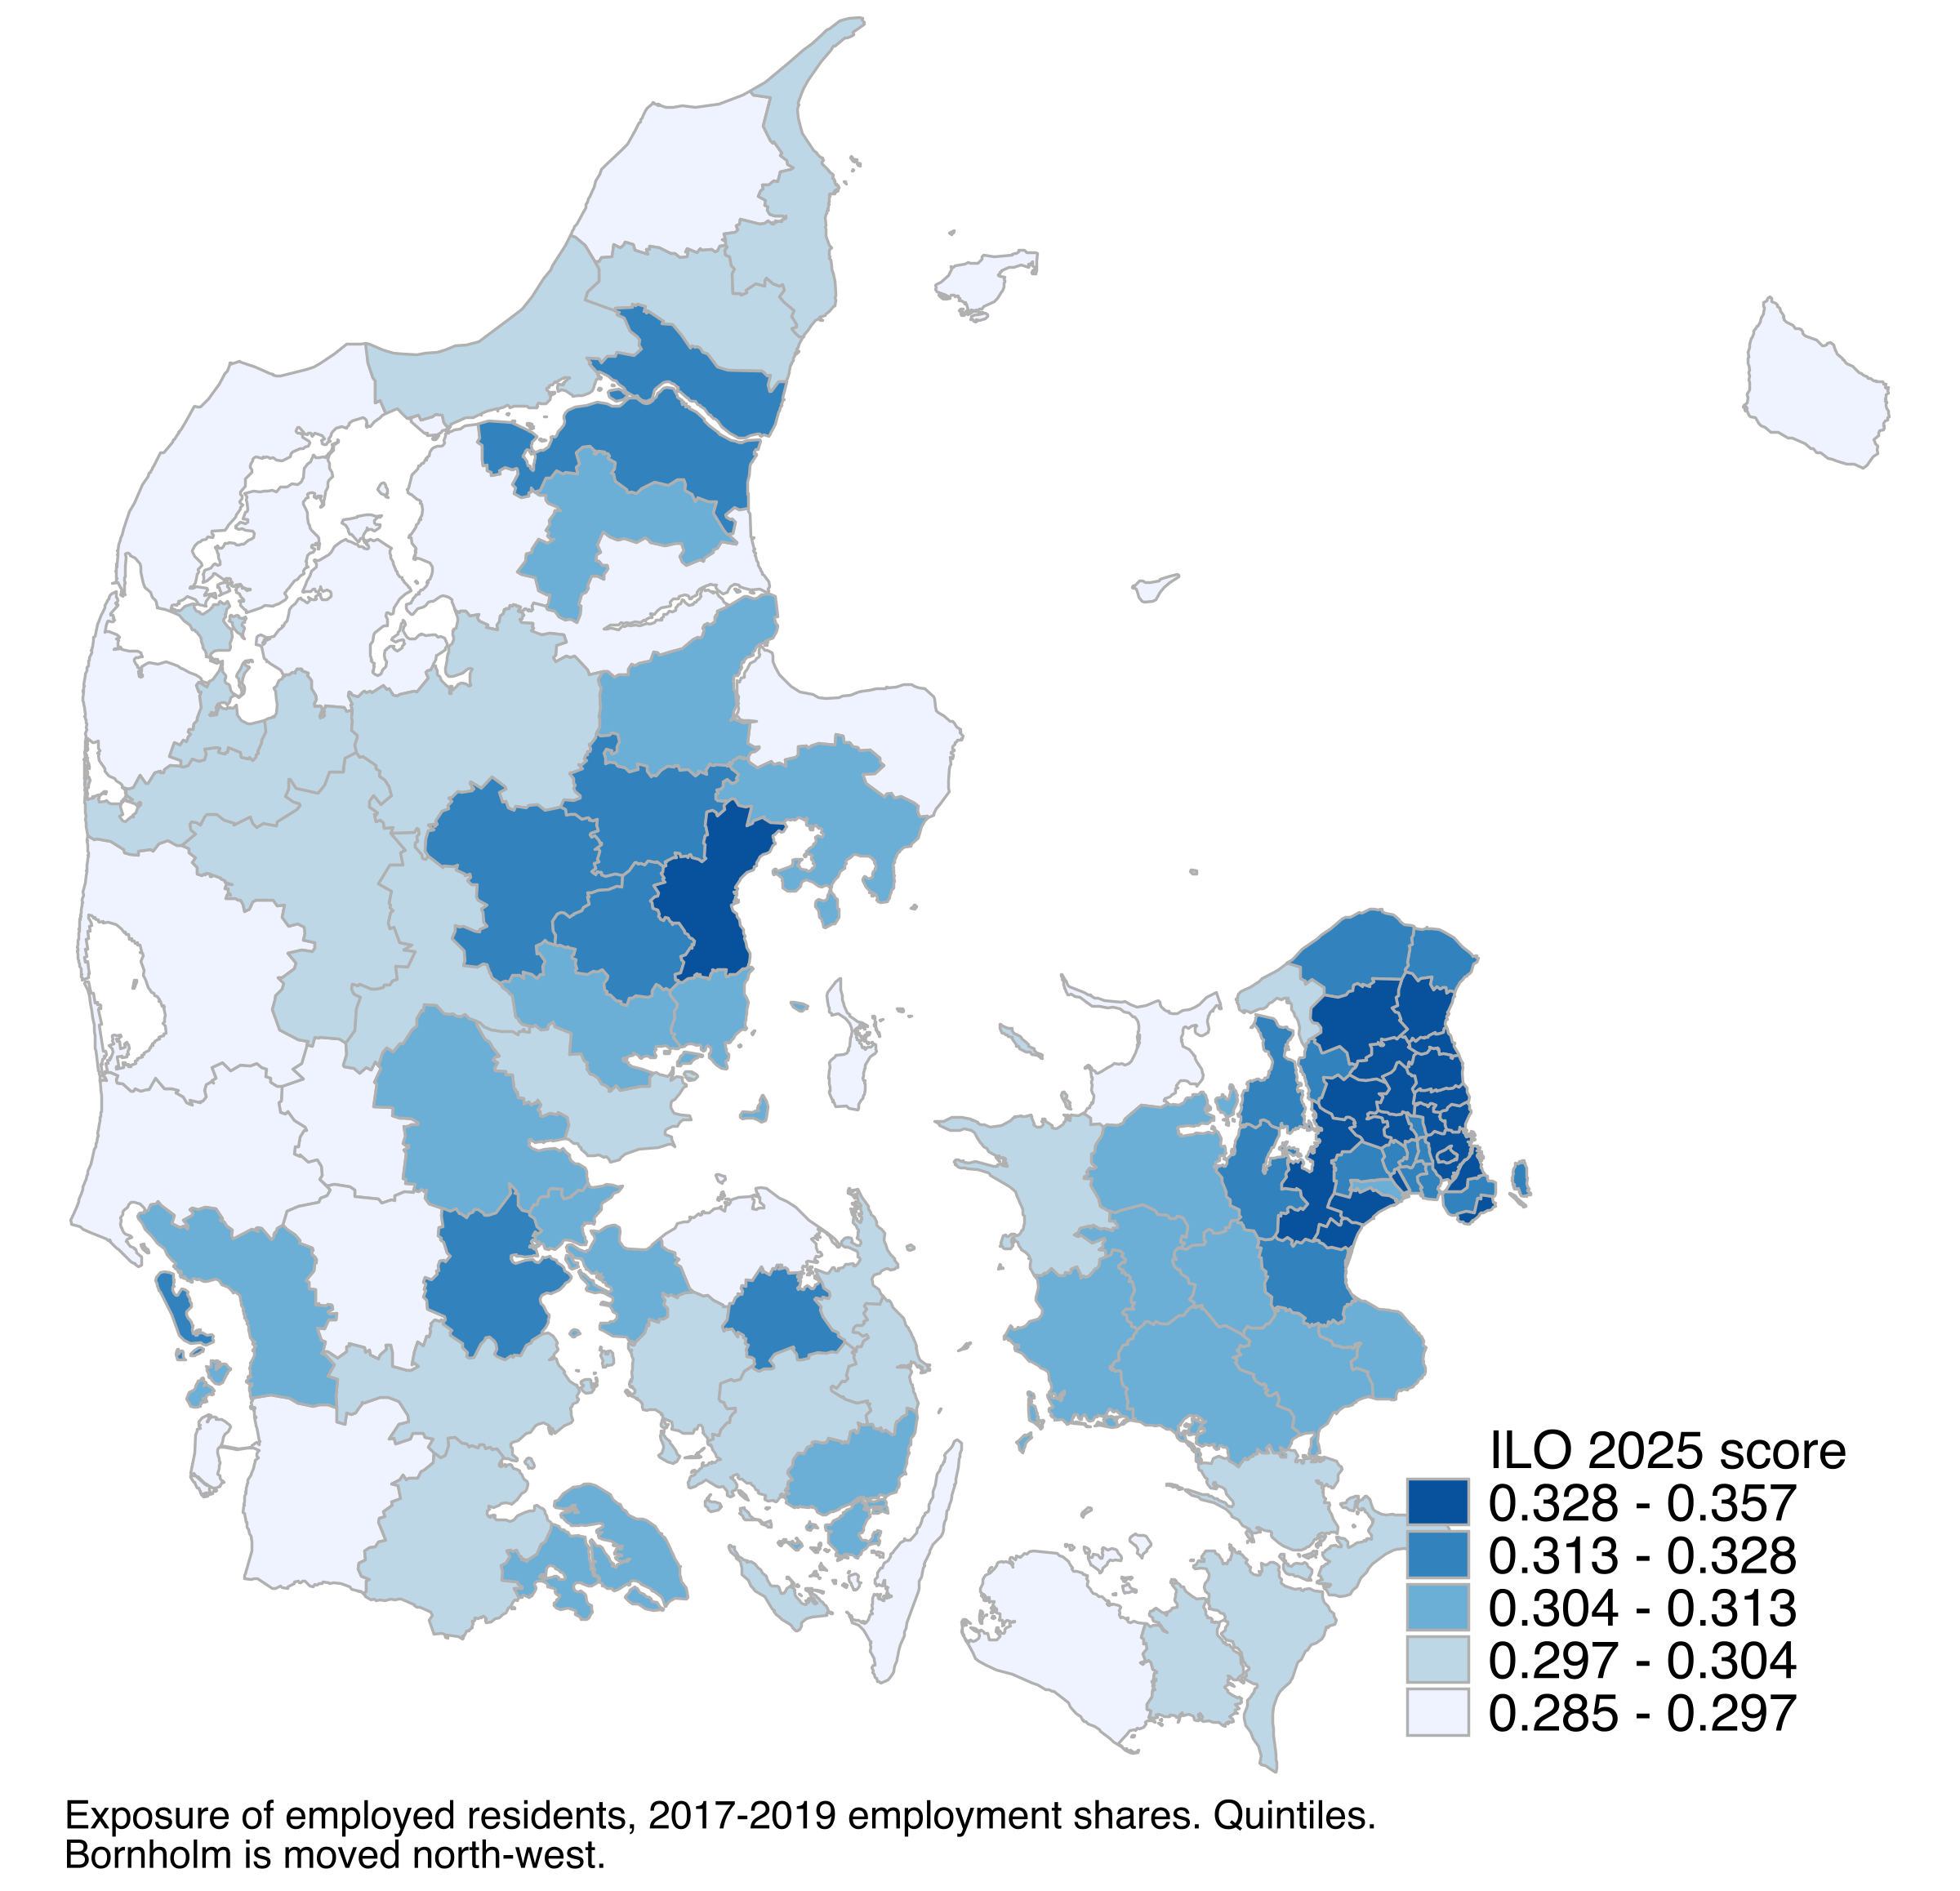
\includegraphics[width=0.78\textwidth]{map_exposure.png}
\caption{Resident exposure to generative AI by municipality}\label{fig:map}
\begin{minipage}{0.95\textwidth}
\footnotesize \textit{Notes:} Exposure of employed residents, built from ILO 2025 occupation scores and 2017--2019 employment shares by industry and skill level. Quintiles across the 98 municipalities. Bornholm is moved north-west of its true position.
\end{minipage}
\end{figure}

Both dimensions of the measure contribute to this variation. A version that assigns every worker the average score of their industry has a standard deviation of 0.013 and correlates 0.985 with the baseline. A version that assigns every worker the national score of their skill level has a standard deviation of 0.008 and correlates 0.93 with the baseline. Exposure measured at the workplace correlates 0.84 with resident exposure, and exposure based on the 2023 scores correlates 0.99 with the 2025 version.

\subsection{What else differs across exposed municipalities}

Table~\ref{tab:balance} compares exposed and less exposed municipalities on characteristics measured in 2019. Exposure correlates 0.94 with the log price per square metre, 0.92 with the tertiary education share, 0.84 with population density and 0.82 with log income. The most exposed third of municipalities also had faster house price growth from 2015 to 2019, 18 log points against 9 for the least exposed third. Equity holdings relative to income, which determine how much residents gained from the rise in stock prices of AI-related firms after 2022, correlate 0.63 with exposure. Mortgage debt relative to income correlates only 0.21 with exposure. Resident exposure thus summarizes much of what distinguishes the Copenhagen area from the rest of the country. This is the central challenge for identification.

\begin{table}[t]
\centering
\caption{Municipality characteristics by exposure, 2019}\label{tab:balance}
\resizebox{\textwidth}{!}{\begin{tabular}{lccccc}
\toprule
 & Mean & SD & Low exposure & High exposure & Correlation \\
 & & & (bottom tercile) & (top tercile) & with exposure \\
\midrule
Log house price per m2, 2019 &   9.44 &   0.57 &   8.85 &  10.11 &  0.94 \\
House price growth 2015-2019 (log points) &   0.14 &   0.07 &   0.09 &   0.18 &  0.42 \\
Log price per m2 minus log income &  -2.96 &   0.48 &  -3.46 &  -2.41 &  0.86 \\
Log disposable income per person, 2019 &  12.40 &   0.15 &  12.30 &  12.53 &  0.82 \\
Tertiary education share, 15-69 &   0.22 &   0.05 &   0.18 &   0.27 &  0.92 \\
Mortgage debt / disposable income &   1.93 &   0.30 &   1.92 &   2.01 &  0.21 \\
Listed shares and funds / disposable income &   0.50 &   0.27 &   0.42 &   0.67 &  0.63 \\
Log population density &   5.20 &   1.38 &   4.01 &   6.69 &  0.84 \\
Share of dwellings in multi-dwelling buildings &   0.28 &   0.18 &   0.15 &   0.42 &  0.62 \\
Log distance to Copenhagen (km) &   4.33 &   1.22 &   5.27 &   3.07 & -0.77 \\
\bottomrule
\end{tabular}
}
\begin{minipage}{\textwidth}
\footnotesize \smallskip
\textit{Notes:} 98 municipalities. Low and high exposure are the bottom and top terciles of standardized resident exposure. The last column reports the correlation with standardized exposure. Mortgage debt, equity holdings and income are averages per adult and per person.
\end{minipage}
\end{table}

%-------------------------------------------------------------------------------
\section{Empirical Strategy}\label{sec:strategy}
%-------------------------------------------------------------------------------

\subsection{Long differences}

The first specification compares price growth across municipalities,
\begin{equation}\label{eq:longdiff}
\Delta \ln P_m = \alpha + \beta E_m + X_m'\gamma + \delta_{p(m)} + \varepsilon_m,
\end{equation}
where $\Delta \ln P_m$ is the change in the log price per square metre from the mean of 2021Q4--2022Q3 to the mean of 2025Q3--2026Q2. Averaging over four quarters at each end reduces noise in municipalities with few sales. $X_m$ contains the 2019 characteristics in Table~\ref{tab:balance}, and $\delta_{p(m)}$ are fixed effects for the 11 provinces. A placebo version uses the change from 2014Q4--2015Q3 to 2018Q4--2019Q3, a window of the same length that ends three years before ChatGPT. Standard errors are robust to heteroskedasticity.

\subsection{Event study}

The second specification traces relative prices quarter by quarter,
\begin{equation}\label{eq:es}
\ln P_{mt} = \alpha_m + \delta_{p(m),t} + \sum_{k \neq 2022Q3} \beta_k \, E_m \, \mathbf{1}[t = k] + \sum_k X_m'\gamma_k \, \mathbf{1}[t = k] + \varepsilon_{mt},
\end{equation}
for 2015Q1--2026Q2. Municipality fixed effects $\alpha_m$ absorb permanent price differences. Province-by-quarter fixed effects $\delta_{p(m),t}$ restrict comparisons to municipalities in the same province and quarter. Baseline characteristics interacted with quarter dummies allow prices to evolve differently by price level, income, education, debt, equity holdings, density, housing type and distance to Copenhagen. The coefficient $\beta_k$ measures how much higher log prices were in quarter $k$, relative to 2022Q3, in a municipality with one standard deviation higher exposure. Coefficients before 2022Q4 test for differential trends. I also report a version with national quarter fixed effects and no controls. Standard errors are clustered by municipality. Bornholm is the only municipality in its province, so province-by-quarter fixed effects absorb it.

\subsection{Identification}

The coefficients identify an effect of generative AI exposure if, absent the technology, prices in more and less exposed municipalities would have moved in parallel after 2022Q3. Section~\ref{sec:exposure} shows why this assumption is demanding. Exposed municipalities are urban, educated and expensive, and they had faster price growth before 2022. They are also more sensitive to interest rates, which rose in 2022 and fell from 2024, and to the 2024 property tax reform. Exposed occupations can often be done from home \citep{dingel2020}, and remote work changed housing demand across locations after 2020 \citep{gupta2022, mondragon2022}. Province-by-quarter fixed effects remove regional shocks, including shocks to regional labor demand, and baseline controls interacted with time absorb differential trends along observed characteristics. The pre-period coefficients and the placebo regressions show whether these adjustments succeed.

%-------------------------------------------------------------------------------
\section{Results}\label{sec:results}
%-------------------------------------------------------------------------------

\subsection{Raw price paths}

Figure~\ref{fig:terciles} plots the mean log price per square metre in each tercile of exposure relative to 2022Q3. The most exposed municipalities gained roughly 20 log points on the least exposed between 2015 and 2021. The three groups then moved together until mid-2022. Between 2022Q2 and early 2023, when interest rates rose, prices fell by about 11 log points in the most exposed tercile and by 6 to 7 log points in the other two. The most exposed tercile recovered more slowly in 2023 and pulled ahead from 2024, when rates began to fall. By 2026Q2, prices in the most exposed tercile were about 21 log points above their 2022Q3 level, against about 10 log points in the other two terciles. The renewed divergence thus starts more than a year after ChatGPT's release and coincides with lower interest rates.

\begin{figure}[t]
\centering
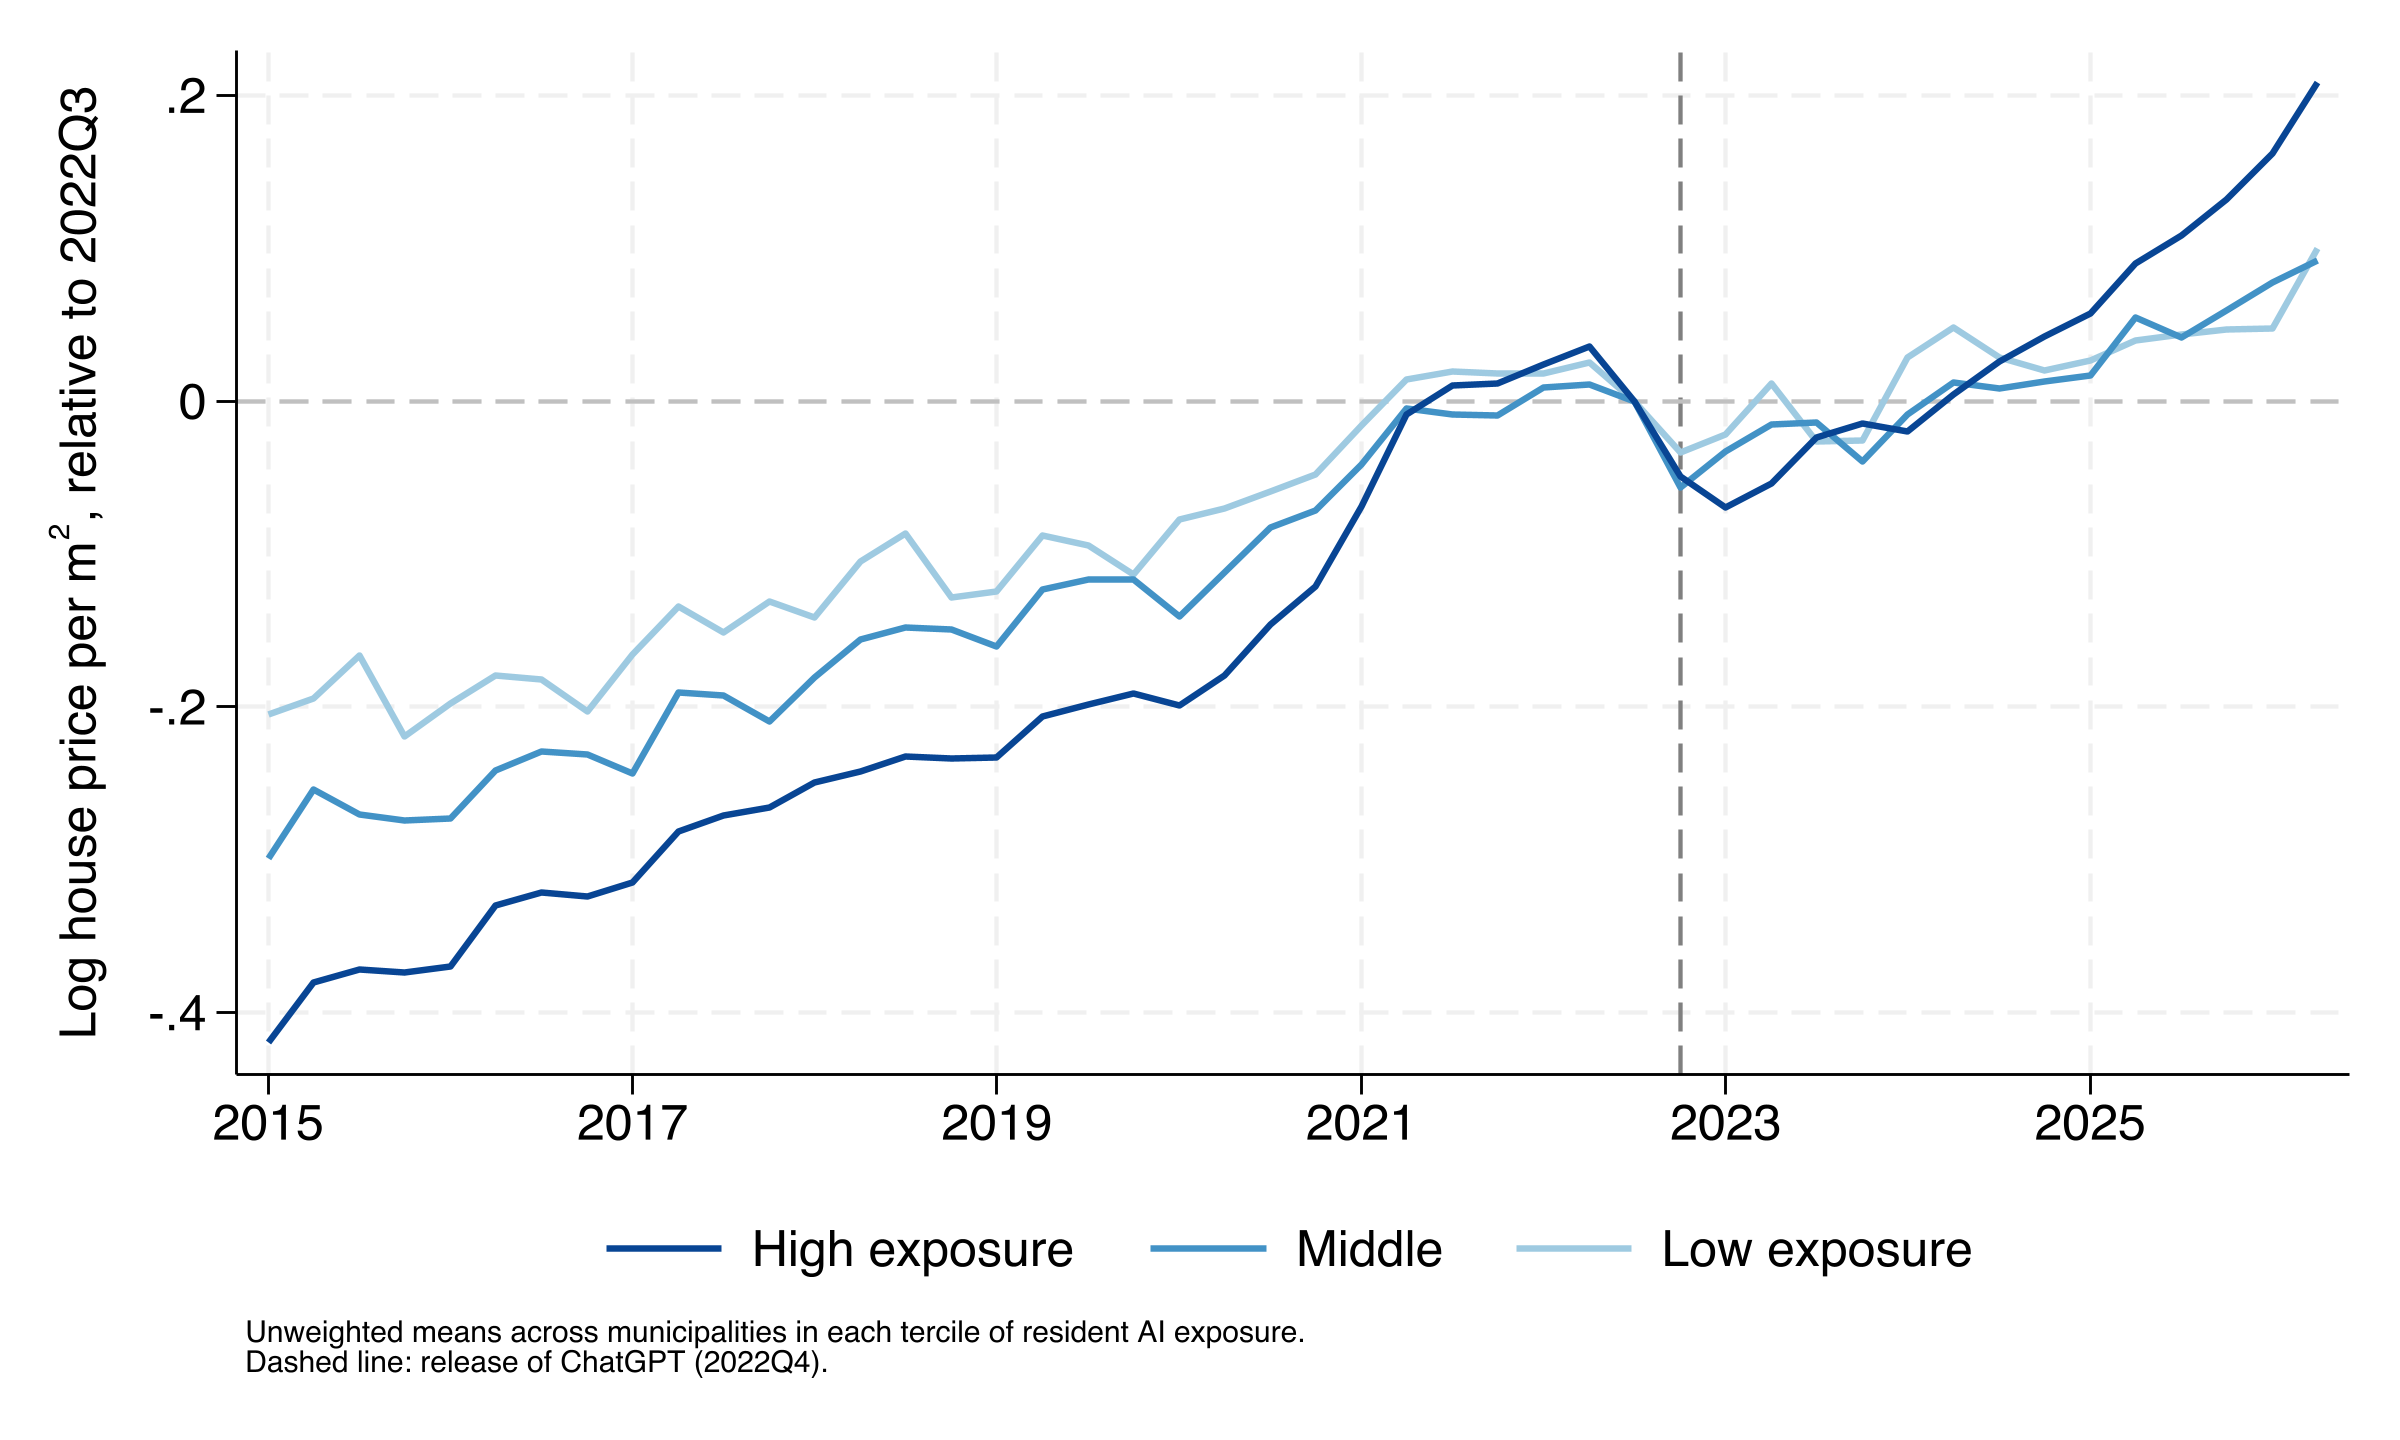
\includegraphics[width=0.9\textwidth]{prices_by_tercile.png}
\caption{House prices by tercile of exposure}\label{fig:terciles}
\begin{minipage}{0.95\textwidth}
\footnotesize \textit{Notes:} Unweighted mean across municipalities of the log realized price per square metre for houses, relative to each municipality's 2022Q3 value. Terciles of standardized resident exposure. The dashed line marks the release of ChatGPT.
\end{minipage}
\end{figure}

\subsection{Long differences}

Table~\ref{tab:longdiff} reports estimates of equation~\eqref{eq:longdiff}, and Figure~\ref{fig:scatter} plots the raw relationship. Without controls, a one standard deviation increase in exposure is associated with 3.5 log points faster growth in house prices between 2022 and 2026 (column 1). Adding pre-period price growth barely changes the estimate (column 2). The placebo regression in column 8 shows the same association, 3.4 log points, for 2015--2019. The cross-sectional association between exposure and price growth therefore predates generative AI.

\begin{table}[t]
\centering
\caption{Exposure and house price growth: long differences}\label{tab:longdiff}
\resizebox{\textwidth}{!}{{
\def\sym#1{\ifmmode^{#1}\else\(^{#1}\)\fi}
\begin{tabular}{l*{9}{c}}
\toprule
                    &\multicolumn{1}{c}{(1)}&\multicolumn{1}{c}{(2)}&\multicolumn{1}{c}{(3)}&\multicolumn{1}{c}{(4)}&\multicolumn{1}{c}{(5)}&\multicolumn{1}{c}{(6)}&\multicolumn{1}{c}{(7)}&\multicolumn{1}{c}{(8)}&\multicolumn{1}{c}{(9)}\\
                    &\multicolumn{1}{c}{Houses}&\multicolumn{1}{c}{Houses}&\multicolumn{1}{c}{Houses}&\multicolumn{1}{c}{Houses}&\multicolumn{1}{c}{Houses}&\multicolumn{1}{c}{Excl. Cph}&\multicolumn{1}{c}{Flats}&\multicolumn{1}{c}{Placebo}&\multicolumn{1}{c}{Placebo}\\
\midrule
AI exposure, residents (standardized)&       0.035\sym{***}&       0.032\sym{***}&       0.008         &       0.045\sym{*}  &       0.055         &       0.057         &       0.001         &       0.034\sym{***}&       0.001         \\
                    &     (0.006)         &     (0.006)         &     (0.010)         &     (0.027)         &     (0.034)         &     (0.035)         &     (0.079)         &     (0.007)         &     (0.011)         \\
\addlinespace
House price growth 2015-2019 (log points)&                     &       0.111\sym{*}  &                     &      -0.103         &      -0.080         &      -0.097         &       0.337         &                     &                     \\
                    &                     &     (0.066)         &                     &     (0.092)         &     (0.121)         &     (0.122)         &     (0.495)         &                     &                     \\
\addlinespace
Baseline controls   &          No         &          No         &          No         &         Yes         &         Yes         &         Yes         &         Yes         &          No         &          No         \\
\addlinespace
Province FE         &          No         &          No         &         Yes         &          No         &         Yes         &         Yes         &         Yes         &          No         &         Yes         \\
\midrule
Municipalities      &          98         &          98         &          98         &          98         &          98         &          96         &          73         &          98         &          98         \\
R-squared           &        0.28         &        0.29         &        0.46         &        0.47         &        0.53         &        0.54         &        0.33         &        0.19         &        0.53         \\
\bottomrule
\end{tabular}
}
}
\begin{minipage}{\textwidth}
\footnotesize \smallskip
\textit{Notes:} The dependent variable in columns 1--7 is the change in the log realized price per square metre from the mean of 2021Q4--2022Q3 to the mean of 2025Q3--2026Q2. In columns 8--9 it is the change from 2014Q4--2015Q3 to 2018Q4--2019Q3. Exposure is standardized resident exposure. Baseline controls are the 2019 log price, log income, tertiary education share, mortgage debt and equity holdings relative to income, log density, share of multi-dwelling buildings and log distance to Copenhagen. Column 6 excludes Copenhagen and Frederiksberg. Column 7 uses owner-occupied flats. Robust standard errors in parentheses. * $p<0.10$, ** $p<0.05$, *** $p<0.01$.
\end{minipage}
\end{table}

\begin{figure}[t]
\centering
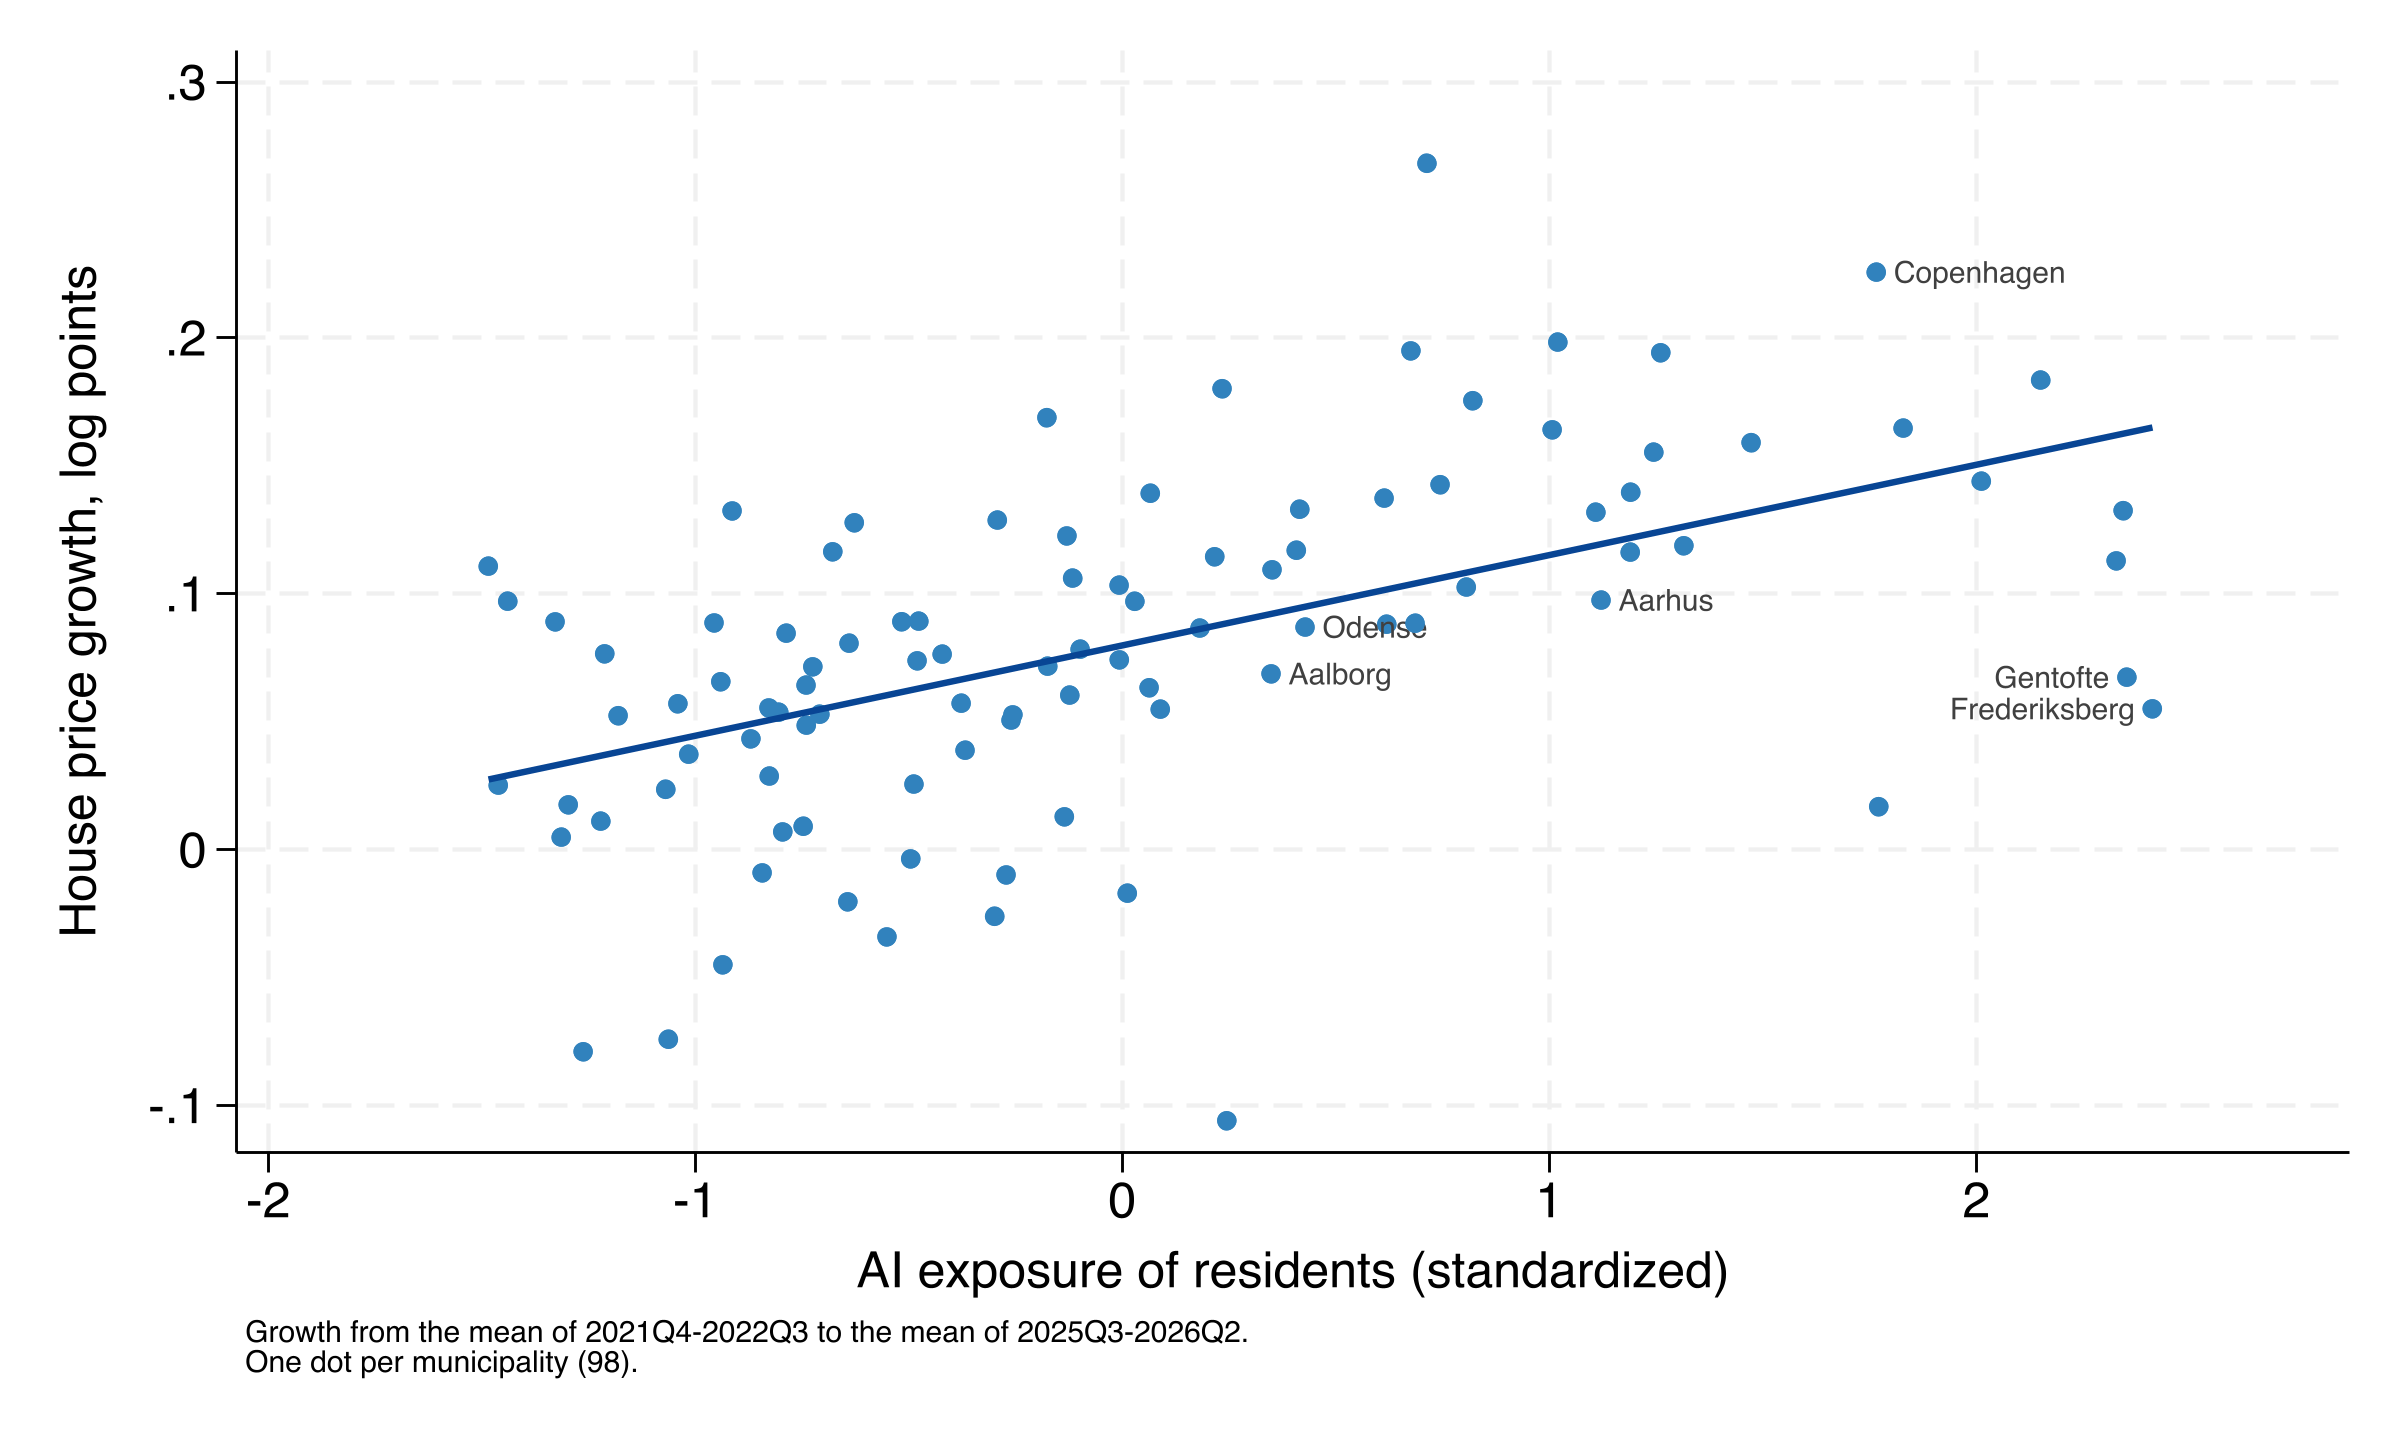
\includegraphics[width=0.9\textwidth]{longdiff_scatter.png}
\caption{Exposure and house price growth, 2022--2026}\label{fig:scatter}
\begin{minipage}{0.95\textwidth}
\footnotesize \textit{Notes:} Change in the log realized price per square metre for houses from the mean of 2021Q4--2022Q3 to the mean of 2025Q3--2026Q2 against standardized resident exposure. One observation per municipality, with a linear fit.
\end{minipage}
\end{figure}

Province fixed effects remove the association in both periods. Within provinces, the coefficient falls to 0.8 log points with a standard error of 1.0 after ChatGPT (column 3) and to 0.1 log points in the placebo period (column 9). Adding the baseline controls raises the point estimate to 4.5 log points without province effects and 5.5 log points with them (columns 4 and 5), but the standard errors rise to 2.7 and 3.4. This instability reflects the near-collinearity of exposure with the price level and education. Once these characteristics enter the regression, little independent variation in exposure remains, and the estimate depends on which controls are included. Excluding Copenhagen and Frederiksberg leaves the estimate unchanged (column 6). For flats, the estimate is 0.1 log points with a standard error of 7.9 (column 7).

\subsection{Event study}

Figure~\ref{fig:es} plots the event-study coefficients, and Table~\ref{tab:es} averages them over four periods. With national quarter fixed effects, the coefficients rise steadily from $-6.6$ log points in 2015--2019 to $-2.1$ in 2020--2022Q2 and to 1.5 in 2024--2026Q2. This path reflects the faster growth of exposed municipalities throughout the sample, not a break at the end of 2022. The slope is about 1.2 log points per year before 2022 and about 0.6 afterward, so relative growth in exposed municipalities slowed rather than accelerated after ChatGPT.

\begin{figure}[t]
\centering
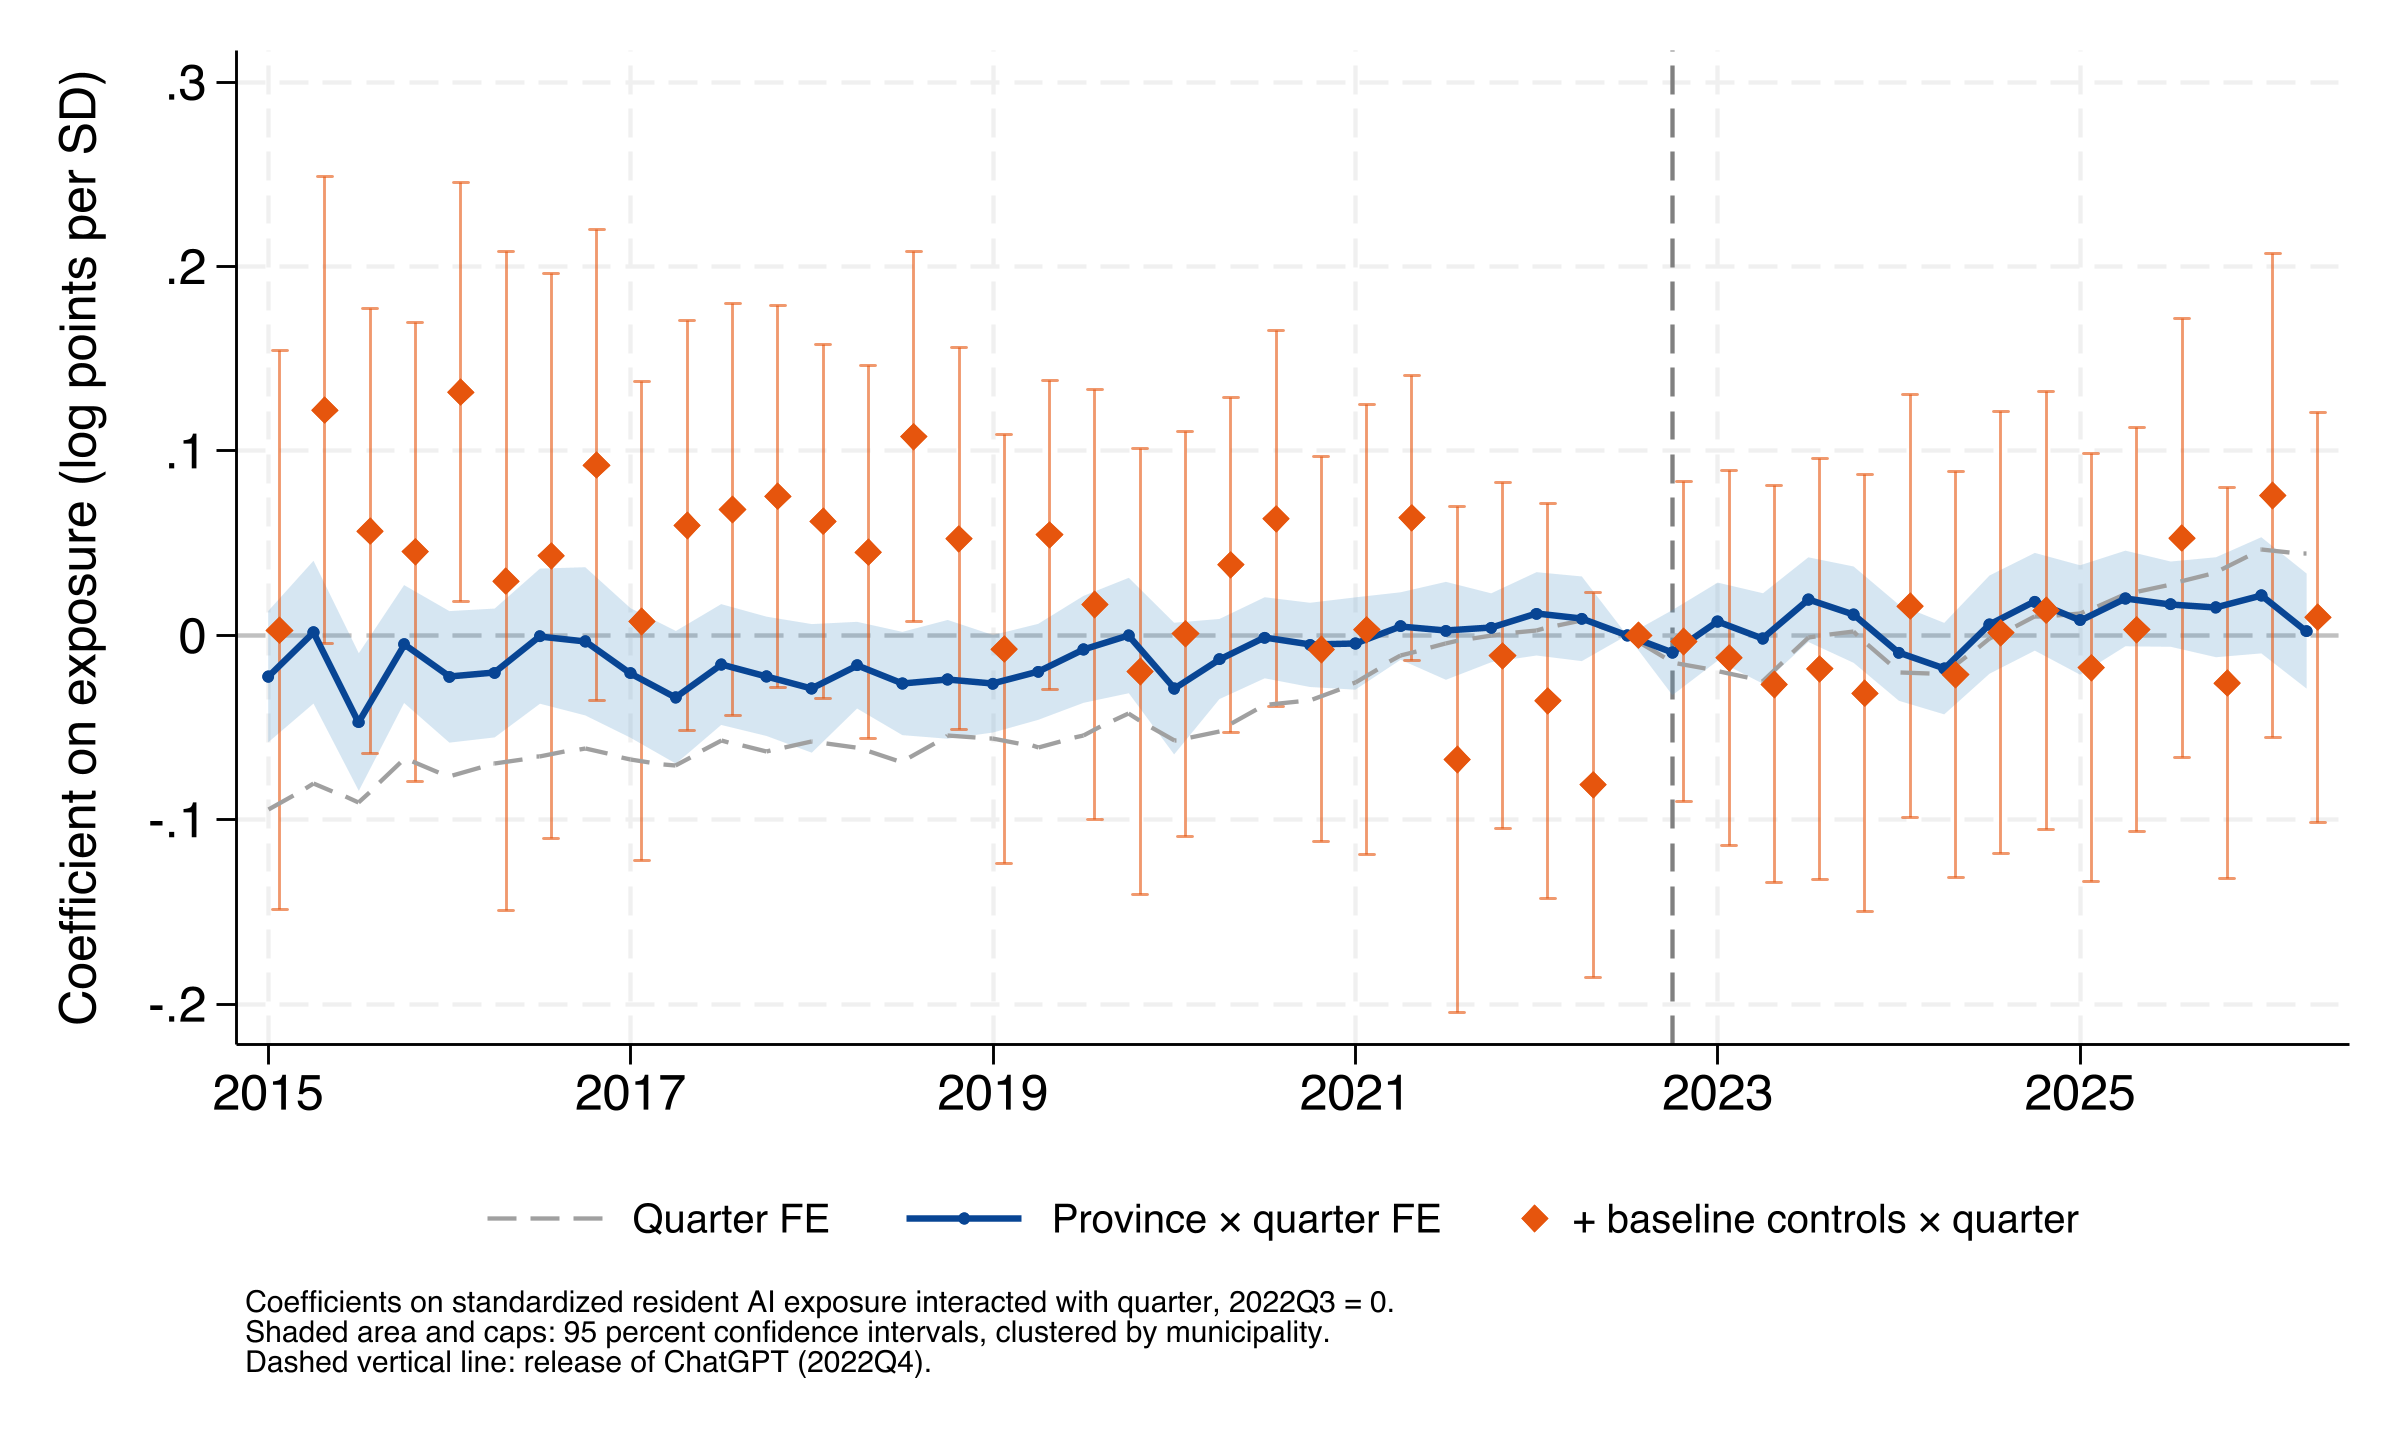
\includegraphics[width=0.95\textwidth]{eventstudy.png}
\caption{Event study: house prices and exposure to generative AI}\label{fig:es}
\begin{minipage}{0.95\textwidth}
\footnotesize \textit{Notes:} Coefficients $\beta_k$ from equation~\eqref{eq:es}, with 2022Q3 normalized to zero. The dashed grey line uses municipality and quarter fixed effects. The blue line adds province-by-quarter fixed effects, and the orange markers add 2019 baseline characteristics interacted with quarter dummies. Shaded area and caps show 95 percent confidence intervals clustered by municipality.
\end{minipage}
\end{figure}

\begin{table}[t]
\centering
\begin{threeparttable}
\caption{Event-study coefficients averaged by period}\label{tab:es}
\small
\begin{tabular}{lccc}
\toprule
 & (1) & (2) & (3) \\
\midrule
2015-2019 & -0.066\sym{***} & -0.018 & 0.052 \\
 & (0.010) & (0.014) & (0.051) \\
2020-2022Q2 & -0.021\sym{***} & -0.002 & -0.003 \\
 & (0.007) & (0.008) & (0.044) \\
2022Q4-2023 & -0.012 & 0.005 & -0.018 \\
 & (0.007) & (0.010) & (0.046) \\
2024-2026Q2 & 0.015\sym{**} & 0.008 & 0.011 \\
 & (0.008) & (0.010) & (0.049) \\
\midrule
Municipality FE & Yes & Yes & Yes \\
Quarter FE & Yes & & \\
Province $\times$ quarter FE & & Yes & Yes \\
Baseline controls $\times$ quarter & & & Yes \\
Observations &  4,483 &  4,437 &  4,437 \\
Municipalities &     98 &     97 &     97 \\
\bottomrule
\end{tabular}

\begin{tablenotes}[flushleft]
\footnotesize
\item \textit{Notes:} Averages of the quarterly coefficients $\beta_k$ from equation~\eqref{eq:es} within each period, relative to 2022Q3. The dependent variable is the log realized price per square metre for houses, 2015Q1--2026Q2. Baseline controls are those in Table~\ref{tab:longdiff}. Standard errors clustered by municipality in parentheses. * $p<0.10$, ** $p<0.05$, *** $p<0.01$.
\end{tablenotes}
\end{threeparttable}
\end{table}

Province-by-quarter fixed effects flatten the path. The average coefficient is $-1.8$ log points with a standard error of 1.4 in 2015--2019 and $-0.2$ in 2020--2022Q2. After ChatGPT it is 0.5 log points in 2022Q4--2023 and 0.8 in 2024--2026Q2, with standard errors of 1.0. None of these averages differs from zero, and no quarterly coefficient after 2022Q3 does either. Adding baseline controls interacted with time yields coefficients that move between $-8$ and 13 log points with standard errors around 6, which leaves the specification uninformative.

\subsection{Magnitudes}

The cross-sectional association is economically large but not specific to generative AI. At the median municipal price of 12,930 DKK per square metre in 2022Q3, a 140 square metre house cost about 1.8 million DKK. The 3.5 log point association in column 1 of Table~\ref{tab:longdiff} corresponds to about 65,000 DKK per standard deviation of exposure over four years, or 44 percent of average growth. The placebo association for 2015--2019 has the same size. Within provinces, the 95 percent confidence interval for the post-ChatGPT coefficient runs from $-1.1$ to 2.7 log points. The upper bound corresponds to about 50,000 DKK for the same house, or a third of average growth. The data can therefore rule out large within-province effects but not modest ones.

%-------------------------------------------------------------------------------
\section{Discussion and Next Steps}\label{sec:discussion}
%-------------------------------------------------------------------------------

The absence of a within-province effect has three possible explanations, which the current design cannot yet distinguish. First, generative AI may not yet have changed expected earnings enough to move housing demand. This reading fits the small labor market effects that \citet{humlum2025} find in Danish administrative data. Second, any effect may run through regional labor demand rather than residential choice. Province-by-quarter fixed effects absorb such an effect, and the remaining between-province variation is too thin, with 11 provinces, and too confounded with the Copenhagen premium to identify it. Third, measurement error in exposure attenuates the estimates. The industry and skill-level cells miss differences in occupation mix within cells, such as the concentration of headquarters functions in Copenhagen.

The analysis so far also leaves several threats unaddressed. The price per square metre is not adjusted for quality, and comparing province aggregates of BM010 with Statistics Denmark's quality-adjusted index EJ56 would show whether changes in the composition of sales matter. Inference does not yet account for correlation across municipalities with similar industry composition \citep{adao2019}. The pre-period coefficients could be used to bound violations of parallel trends \citep{rambachan2023}.

The next version of the paper will extend the analysis in four directions. First, it will split exposure into occupations with augmentation and automation potential \citep{gmyrek2023, pizzinelli2023}. Under the hypothesis, augmentation exposure should raise prices and automation exposure should not. Second, a teleworkability measure built in the same way \citep{dingel2020} will test whether exposure merely proxies for remote work. Third, interacting time with baseline price-to-income and debt-to-income ratios will absorb sensitivity to interest rates, which matters because the post-2024 divergence coincides with rate cuts. Fourth, exposure measured at the workplace and weighted by commuting flows will capture the labor demand channel. With access to Danish register data, occupation counts by municipality and quality-adjusted price indices would remove the two main sources of measurement error.

%-------------------------------------------------------------------------------
\section{Conclusion}\label{sec:conclusion}
%-------------------------------------------------------------------------------

This paper asks whether house prices grew faster in Danish municipalities whose residents work in occupations more exposed to generative AI. Across all municipalities they did, by 3.5 log points per standard deviation of exposure between 2022 and 2026. The same association holds for 2015--2019, and it disappears when municipalities are compared within provinces. Exposure to generative AI, measured from public data, largely captures the long-running premium of educated urban municipalities. Through mid-2026, the Danish housing market shows no sign that it has priced the technology into the relative value of places, and the data rule out within-province effects larger than about 3 log points per standard deviation. Whether capitalization emerges as the labor market effects of generative AI become clearer is a question for future data.

\newpage
\bibliographystyle{aer}
\bibliography{references}

\newpage
\appendix

%-------------------------------------------------------------------------------
\section{Data Sources}\label{app:data}
%-------------------------------------------------------------------------------

Table~\ref{tab:sources} lists the data. Statistics Denmark tables are downloaded through the StatBank API (api.statbank.dk). BM010 is downloaded from the Finans Danmark statistics bank (rkr.statistikbank.dk). The ILO scores are from the repository accompanying \citet{gmyrek2025}, and municipality boundaries are from GADM version 4.1. A single script downloads all data and reproduces every table and figure in the paper.

\begin{table}[h]
\centering
\caption{Data sources}\label{tab:sources}
\resizebox{\textwidth}{!}{%
\begin{tabular}{lll}
\toprule
Source & Content & Coverage \\
\midrule
Finans Danmark BM010 & Price per m$^2$ of completed sales, houses and flats & 98 municipalities, 1992Q1--2026Q2 \\
Statistics Denmark RAS302 & Employed residents by industry and status & 98 municipalities, 2008--2024 \\
Statistics Denmark RAS301 & Jobs by industry and status & 98 municipalities, 2008--2024 \\
Statistics Denmark LONS20 & Full-time employees by 4-digit DISCO and sector & National, 2013--2025 \\
Statistics Denmark FRA029 & Full-time employed by industry and DISCO major group & National, 2013--2024 \\
Statistics Denmark FRA020 & Full-time employed by sector and 2-digit DISCO & National, 2013--2024 \\
Statistics Denmark FOLK1A & Population & 98 municipalities, quarterly \\
Statistics Denmark ARE207 & Land area & 98 municipalities \\
Statistics Denmark INDKP101 & Disposable income per person & 98 municipalities, 1987--2025 \\
Statistics Denmark HFUDD11 & Educational attainment, 15--69 year olds & 98 municipalities, 2008--2025 \\
Statistics Denmark FORMUE12 & Wealth and debt per adult & 98 municipalities, 2014--2024 \\
Statistics Denmark BOL101 & Dwellings by building type & 98 municipalities, 2010--2026 \\
\citet{gmyrek2025} & GenAI exposure of tasks and occupations & 427 ISCO-08 unit groups \\
GADM 4.1 & Municipality boundaries & 98 municipalities \\
\bottomrule
\end{tabular}}
\end{table}

%-------------------------------------------------------------------------------
\section{Alternative Exposure Measures}\label{app:measures}
%-------------------------------------------------------------------------------

\begin{table}[h]
\centering
\caption{Distribution of exposure across municipalities}\label{tab:variation}
\resizebox{\textwidth}{!}{{
\def\sym#1{\ifmmode^{#1}\else\(^{#1}\)\fi}
\begin{tabular}{l*{1}{ccccccc}}
\toprule
                    &        Mean&          SD&         P10&         P50&         P90&         Min&         Max\\
\midrule
AI exposure, residents (ILO 2025, industry and skill level)&       0.312&       0.019&       0.290&       0.309&       0.340&       0.285&       0.357\\
AI exposure, residents (industry only)&       0.318&       0.013&       0.302&       0.314&       0.336&       0.297&       0.352\\
AI exposure, residents (skill level only)&       0.317&       0.008&       0.308&       0.315&       0.327&       0.302&       0.335\\
AI exposure, jobs in municipality (ILO 2025, industry and skill level)&       0.308&       0.018&       0.289&       0.304&       0.337&       0.283&       0.360\\
AI exposure, residents (ILO 2023)&       0.320&       0.017&       0.300&       0.318&       0.346&       0.293&       0.360\\
\bottomrule
\end{tabular}
}
}
\begin{minipage}{\textwidth}
\footnotesize \smallskip
\textit{Notes:} 98 municipalities. The baseline measure weights industry-by-skill cell scores by the 2017--2019 employment of residents. The industry-only and skill-only versions assign every worker the average score of their industry or the national score of their skill level. The workplace version weights by jobs located in the municipality.
\end{minipage}
\end{table}

\end{document}
